\begin{frame}[fragile]{Schema del database \href{https://en.wikiversity.org/wiki/Database_Examples/Northwind/MySQL}{\underline{Northwind}}}
\begin{figure}
    \centering
    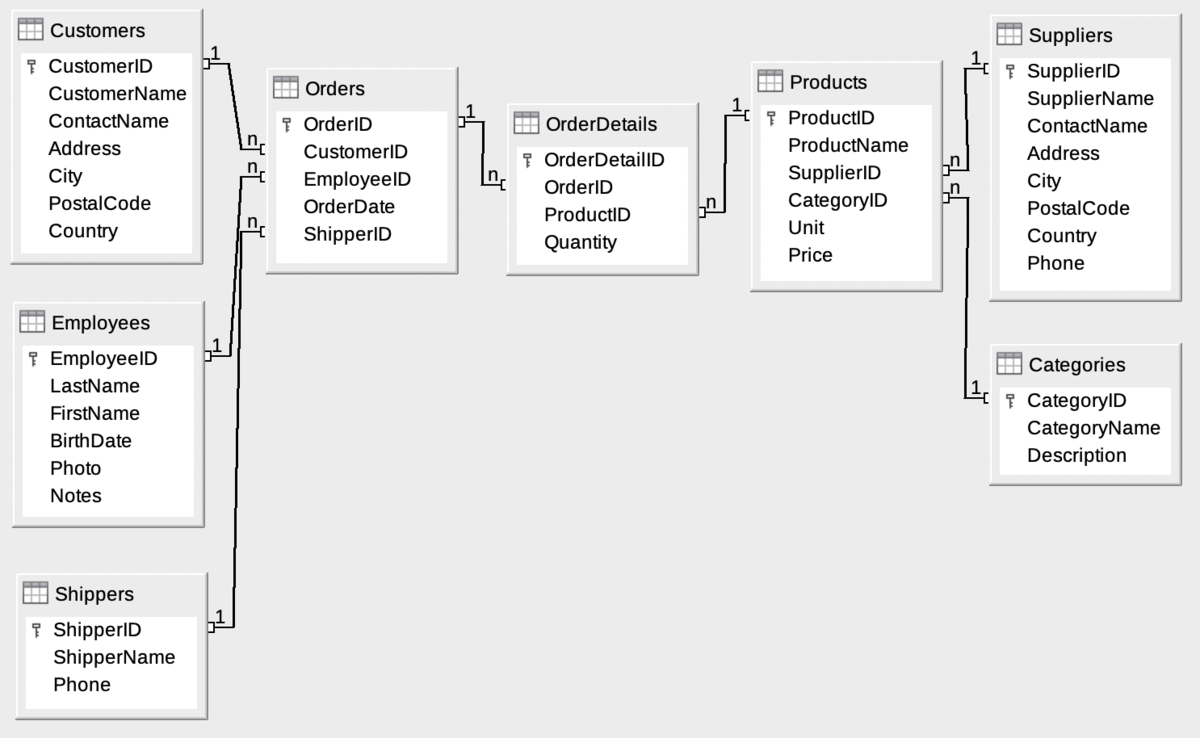
\includegraphics[width=.7\textwidth]{img/db-northwind.png}
\end{figure}
\end{frame}
%
\begin{frame}[fragile]{Northwind: Es. 1}
Mostra nome e categoria dei prodotti con prezzo superiore a 15.
\pause
\begin{lstlisting}
SELECT p.ProductName, c.CategoryName, p.Price
FROM Products AS p
JOIN Categories AS c ON p.CategoryID = c.CategoryID
WHERE p.Price > 15;
\end{lstlisting}
\end{frame}
%
\begin{frame}[fragile]{Northwind: Es. 2}
Conta quanti ordini sono stati spediti da ogni corriere.
\pause
\begin{lstlisting}
SELECT s.ShipperName, COUNT(*) AS TotalOrders
FROM Orders AS o
JOIN Shippers AS s ON o.ShipperID = s.ShipperID
GROUP BY s.ShipperID;
\end{lstlisting}
\end{frame}
%
\begin{frame}[fragile]{Northwind: Es. 3}
Elenca il nome dei clienti e il nome dei dipendenti associati allo stesso ordine.
\pause
\begin{lstlisting}
SELECT o.OrderID, c.CustomerName, 
    e.FirstName AS EmployeeFirstName, 
	e.LastName AS EmployeeLastName
FROM Orders AS o 
JOIN Customers AS c ON o.CustomerID = c.CustomerID
JOIN Employees AS e ON o.EmployeeID = e.EmployeeID;
\end{lstlisting}
\end{frame}
%
\begin{frame}[fragile]{Northwind: Es. 4}
Trova il totale delle quantit\`a ordinate per ogni prodotto.
\pause
\begin{lstlisting}
SELECT p.ProductName, SUM(od.Quantity) AS Quantity
FROM Products AS p
JOIN OrderDetails AS od ON p.ProductID = od.ProductID
GROUP by p.ProductID;
\end{lstlisting}
\end{frame}
%
\begin{frame}[fragile]{Northwind: Es. 5}
Visualizza nome e prezzo dei prodotti il cui prezzo \`e superiore a quello medio di tutti i prodotti.
\pause
\begin{lstlisting}
SELECT ProductName, Price
FROM Products
WHERE Price > (
    SELECT AVG(Price)
    FROM Products
);
\end{lstlisting}
\end{frame}
%
\begin{frame}[fragile]{Northwind: Es. 6}
Elenca i nomi dei clienti che non hanno mai effettuato ordini.
\pause
\newline
\newline
Versione con LEFT JOIN
\begin{lstlisting}
SELECT CustomerName
FROM Customers AS c
LEFT JOIN Orders AS o ON c.CustomerID = o.CustomerID
WHERE o.CustomerID IS NULL;
\end{lstlisting}
\end{frame}

\begin{frame}[fragile]{Northwind: Es. 6}
Elenca i nomi dei clienti che non hanno mai effettuato ordini.
\newline
\newline
Versione con NOT IN
\begin{lstlisting}
SELECT c.CustomerName
FROM Customers as c
WHERE c.CustomerID NOT IN(
	SELECT CustomerID
	FROM Orders
);
\end{lstlisting}
\end{frame}
%
\begin{frame}[fragile]{Northwind: Es. 7}
Trova i nomi dei prodotti forniti da pi\`u fornitori diversi.
\pause
\begin{lstlisting}
SELECT p.ProductName, 
    COUNT(DISTINCT s.SupplierID) AS SupplierCount
FROM Products
GROUP BY p.ProductID
HAVING SupplierCount >= 2;
\end{lstlisting}
\end{frame}
%
\begin{frame}[fragile]{Northwind: Es. 8}
Elenca i nomi le citt\`a in cui si trovano fornitori o clienti.
\pause
\begin{lstlisting}
SELECT City
FROM Customers
UNION
SELECT City
FROM Suppliers;
\end{lstlisting}
\end{frame}
%
\begin{frame}[fragile]{Northwind: Es. 9}
Elenca i nomi le citt\`a in cui si trovano sia fornitori che clienti.
\pause
\begin{lstlisting}
SELECT City
FROM Customers
INTERSECT
SELECT City
FROM Suppliers;
\end{lstlisting}
\end{frame}

\begin{frame}[fragile]{Northwind: Es. 9}
Elenca i nomi le citt\`a in cui si trovano sia fornitori che clienti.
\newline
\newline
Altra soluzione Possibile:
\begin{lstlisting}
SELECT DISTINCT City
FROM Customers
WHERE City IN (
    SELECT City
    FROM Suppliers
);
\end{lstlisting}
\end{frame}
%
\begin{frame}[fragile]{Northwind: Es. 10}
Mostra data, prodotti e quantit\`a degli ordini fatti durante il gennaio del 1997.
Visualizzare gli ordini dal pi\`u al meno recente.
In caso di ordini fatti allo stesso momento, ordinare per quantit\`a.
\pause
\begin{lstlisting}
SELECT o.OrderDate, p.ProductName, od.Quantity
FROM Orders AS o 
JOIN OrderDetails AS od ON o.OrderID = od.OrderID
JOIN Products AS p ON od.ProductID = p.ProductID
WHERE YEAR(o.OrderDate) = 1997 AND MONTH(o.OrderDate) = 01
ORDER BY o.OrderDate DESC, od.Quantity ASC;
\end{lstlisting}
\end{frame}
%
\begin{frame}[fragile]{Northwind: Es. 11}
Trova gli ordini che contengono solo prodotti della stessa categoria.
\pause
\begin{lstlisting}
SELECT od.OrderID
FROM OrderDetails AS od
JOIN Products AS p ON od.ProductID = p.ProductID
GROUP BY od.OrderID
HAVING COUNT(DISTINCT p.CategoryID) = 1;
\end{lstlisting}
\end{frame}
%
\begin{frame}[fragile]{Northwind: Es. 12}
Trova il nome dei clienti che hanno ordinato prodotti di almeno 2 categorie diverse.
\pause
\begin{lstlisting}
SELECT DISTINCT c.CustomerName
FROM OrderDetails AS od
JOIN Products AS p ON od.ProductID = p.ProductID
JOIN Orders AS o ON o.OrderID = od.OrderID
JOIN Customers AS c ON c.CustomerID = o.CustomerID
GROUP BY o.OrderID
HAVING COUNT(DISTINCT p.CategoryID) >= 2;
\end{lstlisting}
\end{frame}
%
\begin{frame}[fragile]{Northwind: Es. 13}
Trova il nome dei clienti che hanno ordinato almeno 2 volte in mesi diversi.
\pause
\begin{lstlisting}
SELECT c.CustomerName, 
    COUNT(DISTINCT MONTH(o.OrderDate)) AS NumMonths
FROM Customers AS c JOIN Orders AS o
	ON c.CustomerID = o.CustomerID
GROUP BY c.CustomerID
HAVING NumMonths >= 2;
\end{lstlisting}
\end{frame}
%
\begin{frame}[fragile]{Northwind: Es. 14}
Inserisci un nuovo ordine per il cliente pi\`u recente (cio\`e l'ultimo che ha effettuato un ordine). 
L'impiegato \`e quello che ha gestito pi\`u ordini, mentre lo speditore \`e quello che ha effettuato 
meno consegne.
\pause
\begin{lstlisting}[basicstyle=\scriptsize\ttfamily]
INSERT INTO orders (...)
VALUES(
    (
        SELECT CustomerID
        FROM orders
        ORDER BY OrderDate DESC
        LIMIT 1
    ),
    ...
);
\end{lstlisting}
La clausola \textbf{VALUES} non pu\`o essere utilizzata se al suo interno andiamo ad applicare query annidate 
alla tabella che vogliamo modificare. Queste istruzioni ritorneranno un errore.
\end{frame}

\begin{frame}[fragile]{Northwind: Es. 14}
Inserisci un nuovo ordine per il cliente pi\`u recente (cio\`e l'ultimo che ha effettuato un ordine). 
L'impiegato \`e quello che ha gestito pi\`u ordini, mentre lo speditore \`e quello che ha effettuato 
meno consegne.
\begin{lstlisting}[basicstyle=\scriptsize\ttfamily]
INSERT INTO Orders(CustomerID, ...)
SELECT
	tmp1.CustomerID,
    ...
FROM
	(SELECT CustomerID
    FROM Orders
    ORDER BY OrderDate DESC
    LIMIT 1) AS tmp1,
    ...
\end{lstlisting}
Utilizzando le tabelle derivate possiamo correttamente prendere i dati necessari per l'INSERT.
\end{frame}

\begin{frame}[fragile]{Northwind: Es. 14}
Inserisci un nuovo ordine per il cliente pi\`u recente (cio\`e l'ultimo che ha effettuato un ordine). 
L'impiegato \`e quello che ha gestito pi\`u ordini, mentre lo speditore \`e quello che ha effettuato 
meno consegne.
\newline
\newline
Versione con le viste:
\begin{lstlisting}[basicstyle=\scriptsize\ttfamily]
CREATE VIEW tmp1 AS
	SELECT CustomerID
    FROM Orders
    ORDER BY OrderDate DESC
    LIMIT 1;

...

INSERT INTO Orders(CustomerID, ...)
SELECT
	tmp1.CustomerID,
    ...
FROM tmp1, ...
\end{lstlisting}
\end{frame}
%
\begin{frame}[fragile]{Northwind: Es. 15}
Aumenta il prezzo del 5\% per i prodotti appartenenti alla stessa categoria del prodotto 'Tofu'.
\pause
\begin{lstlisting}
UPDATE Products
SET Price = Price * 1.05
WHERE CategoryID =(
    SELECT TofuID.CategoryID
    FROM (
        SELECT p1.CategoryID
        FROM Products AS p1
        WHERE p1.ProductName = 'Tofu'
    ) AS TofuID
);
\end{lstlisting}
\end{frame}
%
\begin{frame}[fragile]{Northwind: Es. 16}
Trova i nomi dei prodotti che costano pi\`u di almeno un altro prodotto nella stessa categoria.
\pause
\begin{lstlisting}
SELECT DISTINCT p.ProductName
FROM Products AS p
JOIN Products AS p2 ON p.CategoryID = p2.CategoryID
WHERE p.Price > p2.Price;
\end{lstlisting}
\end{frame}
%
\begin{frame}[fragile]{Northwind: Es. 17}
Trova clienti senza ordini che vivono in una citt\`a dove altri clienti hanno ordinato.
\pause
\begin{lstlisting}
SELECT c.CustomerName
FROM Customers AS c
WHERE c.CustomerID NOT IN (
	SELECT CustomerID
    FROM Orders
) AND c.City IN (
	SELECT DISTINCT c1.City
    FROM Customers AS c1
    JOIN Orders AS o1 ON c1.CustomerID = o1.CustomerID
);
\end{lstlisting}
\end{frame}

\begin{frame}[fragile]{Northwind: Es. 17}
Trova clienti senza ordini che vivono in una citt\`a dove altri clienti hanno ordinato.
\newline
\newline
Altra possibile soluzione:
\begin{lstlisting}
SELECT c.CustomerName
FROM Customers c
LEFT JOIN Orders o ON o.CustomerID = c.CustomerID
WHERE o.OrderID IS NULL
AND c.City IN (
	SELECT DISTINCT c2.City
	FROM Customers c2
	JOIN Orders o2 ON o2.CustomerID = c2.CustomerID
);
\end{lstlisting}
\end{frame}
%
\begin{frame}[fragile]{Northwind: Es. 18}
Trova nome e citt\`a dei clienti che vivono nella stessa citt\`a di almeno 2 altri clienti.
\pause
\begin{lstlisting}
SELECT c.CustomerName, c.City
FROM Customers AS c
WHERE (
	SELECT COUNT(*)
    FROM Customers AS c1
    WHERE c1.City = c.City
    AND c1.CustomerID <> c.CustomerID
) >= 2
ORDER BY c.City;
\end{lstlisting}
\end{frame}

\begin{frame}[fragile]{Northwind: Es. 18}
Trova nome e citt\`a dei clienti che vivono nella stessa citt\`a di almeno 2 altri clienti.
\newline
\newline
Altra possibile soluzione:
\begin{lstlisting}
SELECT c.CustomerName, c.City
FROM Customers AS c
WHERE c.City IN (
	SELECT c1.City
    FROM Customers AS c1
    GROUP BY c1.City
    HAVING COUNT(*) > 2
)
ORDER BY c.City;
\end{lstlisting}
\end{frame}

%
\begin{frame}[fragile]{Northwind: Es. 19}
Trova i prodotti pi\`u costosi di tutti quelli forniti dallo stesso fornitore, ordinati per nome.
\pause
\begin{lstlisting}
SELECT *
FROM Products AS p1
WHERE p1.Price > ALL (
    SELECT p2.Price
    FROM Products AS p2
    WHERE p2.SupplierID = p1.SupplierID 
    AND p2.ProductID <> p1.ProductID
)
ORDER BY p1.ProductName;
\end{lstlisting}
\end{frame}

\begin{frame}[fragile]{Northwind: Es. 19}
Trova i prodotti pi\`u costosi di tutti quelli forniti dallo stesso fornitore, ordinati per nome.
\newline
\newline
Altra possibile soluzione:
\begin{lstlisting}
SELECT *
FROM Products AS p1
WHERE p1.Price = (
    SELECT MAX(p2.Price)
    FROM Products AS p2
    WHERE p2.SupplierID = p1.SupplierID
)
ORDER BY p1.ProductName;
\end{lstlisting}
\end{frame}
%
\begin{frame}[fragile]{Northwind: Es. 20}
Trova i clienti che hanno effettuato pi\`u ordini rispetto alla media dei clienti del loro stesso 
paese ('Country'), mostrando nome, paese e numero di ordini. Ordina per numero di ordini decrescente e paese crescente.
\pause
\begin{lstlisting}[basicstyle=\scriptsize\ttfamily]
SELECT c1.CustomerName, c1.Country, COUNT(o1.OrderID) AS NumOrders
FROM Customers AS c1
JOIN Orders AS o1 ON c1.CustomerID = o1.CustomerID
GROUP BY c1.CustomerID, c1.Country
HAVING COUNT(o1.OrderID) > (
    SELECT AVG(NumOrders2)
    FROM (
        SELECT c2.Country, COUNT(o2.OrderID) AS NumOrders2
        FROM Customers AS c2
        JOIN Orders AS o2 ON c2.CustomerID = o2.CustomerID
        WHERE c2.Country = c1.Country
        GROUP BY c2.CustomerID
    ) AS SubAvg
)
ORDER BY NumOrders DESC, c1.Country ASC;
\end{lstlisting}
\end{frame}